\documentclass[1p]{elsarticle_modified}
%\bibliographystyle{elsarticle-num}

%\usepackage[colorlinks]{hyperref}
%\usepackage{abbrmath_seonhwa} %\Abb, \Ascr, \Acal ,\Abf, \Afrak
\usepackage{amsfonts}
\usepackage{amssymb}
\usepackage{amsmath}
\usepackage{amsthm}
\usepackage{scalefnt}
\usepackage{amsbsy}
\usepackage{kotex}
\usepackage{caption}
\usepackage{subfig}
\usepackage{color}
\usepackage{graphicx}
\usepackage{xcolor} %% white, black, red, green, blue, cyan, magenta, yellow
\usepackage{float}
\usepackage{setspace}
\usepackage{hyperref}

\usepackage{tikz}
\usetikzlibrary{arrows}

\usepackage{multirow}
\usepackage{array} % fixed length table
\usepackage{hhline}

%%%%%%%%%%%%%%%%%%%%%
\makeatletter
\renewcommand*\env@matrix[1][\arraystretch]{%
	\edef\arraystretch{#1}%
	\hskip -\arraycolsep
	\let\@ifnextchar\new@ifnextchar
	\array{*\c@MaxMatrixCols c}}
\makeatother %https://tex.stackexchange.com/questions/14071/how-can-i-increase-the-line-spacing-in-a-matrix
%%%%%%%%%%%%%%%

\usepackage[normalem]{ulem}

\newcommand{\msout}[1]{\ifmmode\text{\sout{\ensuremath{#1}}}\else\sout{#1}\fi}
%SOURCE: \msout is \stkout macro in https://tex.stackexchange.com/questions/20609/strikeout-in-math-mode

\newcommand{\cancel}[1]{
	\ifmmode
	{\color{red}\msout{#1}}
	\else
	{\color{red}\sout{#1}}
	\fi
}

\newcommand{\add}[1]{
	{\color{blue}\uwave{#1}}
}

\newcommand{\replace}[2]{
	\ifmmode
	{\color{red}\msout{#1}}{\color{blue}\uwave{#2}}
	\else
	{\color{red}\sout{#1}}{\color{blue}\uwave{#2}}
	\fi
}

\newcommand{\Sol}{\mathcal{S}} %segment
\newcommand{\D}{D} %diagram
\newcommand{\A}{\mathcal{A}} %arc


%%%%%%%%%%%%%%%%%%%%%%%%%%%%%5 test

\def\sl{\operatorname{\textup{SL}}(2,\Cbb)}
\def\psl{\operatorname{\textup{PSL}}(2,\Cbb)}
\def\quan{\mkern 1mu \triangleright \mkern 1mu}

\theoremstyle{definition}
\newtheorem{thm}{Theorem}[section]
\newtheorem{prop}[thm]{Proposition}
\newtheorem{lem}[thm]{Lemma}
\newtheorem{ques}[thm]{Question}
\newtheorem{cor}[thm]{Corollary}
\newtheorem{defn}[thm]{Definition}
\newtheorem{exam}[thm]{Example}
\newtheorem{rmk}[thm]{Remark}
\newtheorem{alg}[thm]{Algorithm}

\newcommand{\I}{\sqrt{-1}}
\begin{document}

%\begin{frontmatter}
%
%\title{Boundary parabolic representations of knots up to 8 crossings}
%
%%% Group authors per affiliation:
%\author{Yunhi Cho} 
%\address{Department of Mathematics, University of Seoul, Seoul, Korea}
%\ead{yhcho@uos.ac.kr}
%
%
%\author{Seonhwa Kim} %\fnref{s_kim}}
%\address{Center for Geometry and Physics, Institute for Basic Science, Pohang, 37673, Korea}
%\ead{ryeona17@ibs.re.kr}
%
%\author{Hyuk Kim}
%\address{Department of Mathematical Sciences, Seoul National University, Seoul 08826, Korea}
%\ead{hyukkim@snu.ac.kr}
%
%\author{Seokbeom Yoon}
%\address{Department of Mathematical Sciences, Seoul National University, Seoul, 08826,  Korea}
%\ead{sbyoon15@snu.ac.kr}
%
%\begin{abstract}
%We find all boundary parabolic representation of knots up to 8 crossings.
%
%\end{abstract}
%\begin{keyword}
%    \MSC[2010] 57M25 
%\end{keyword}
%
%\end{frontmatter}

%\linenumbers
%\tableofcontents
%
\newcommand\colored[1]{\textcolor{white}{\rule[-0.35ex]{0.8em}{1.4ex}}\kern-0.8em\color{red} #1}%
%\newcommand\colored[1]{\textcolor{white}{ #1}\kern-2.17ex	\textcolor{white}{ #1}\kern-1.81ex	\textcolor{white}{ #1}\kern-2.15ex\color{red}#1	}

{\Large $\underline{12a_{0667}~(K12a_{0667})}$}

\setlength{\tabcolsep}{10pt}
\renewcommand{\arraystretch}{1.6}
\vspace{1cm}\begin{tabular}{m{100pt}>{\centering\arraybackslash}m{274pt}}
\multirow{5}{120pt}{
	\centering
	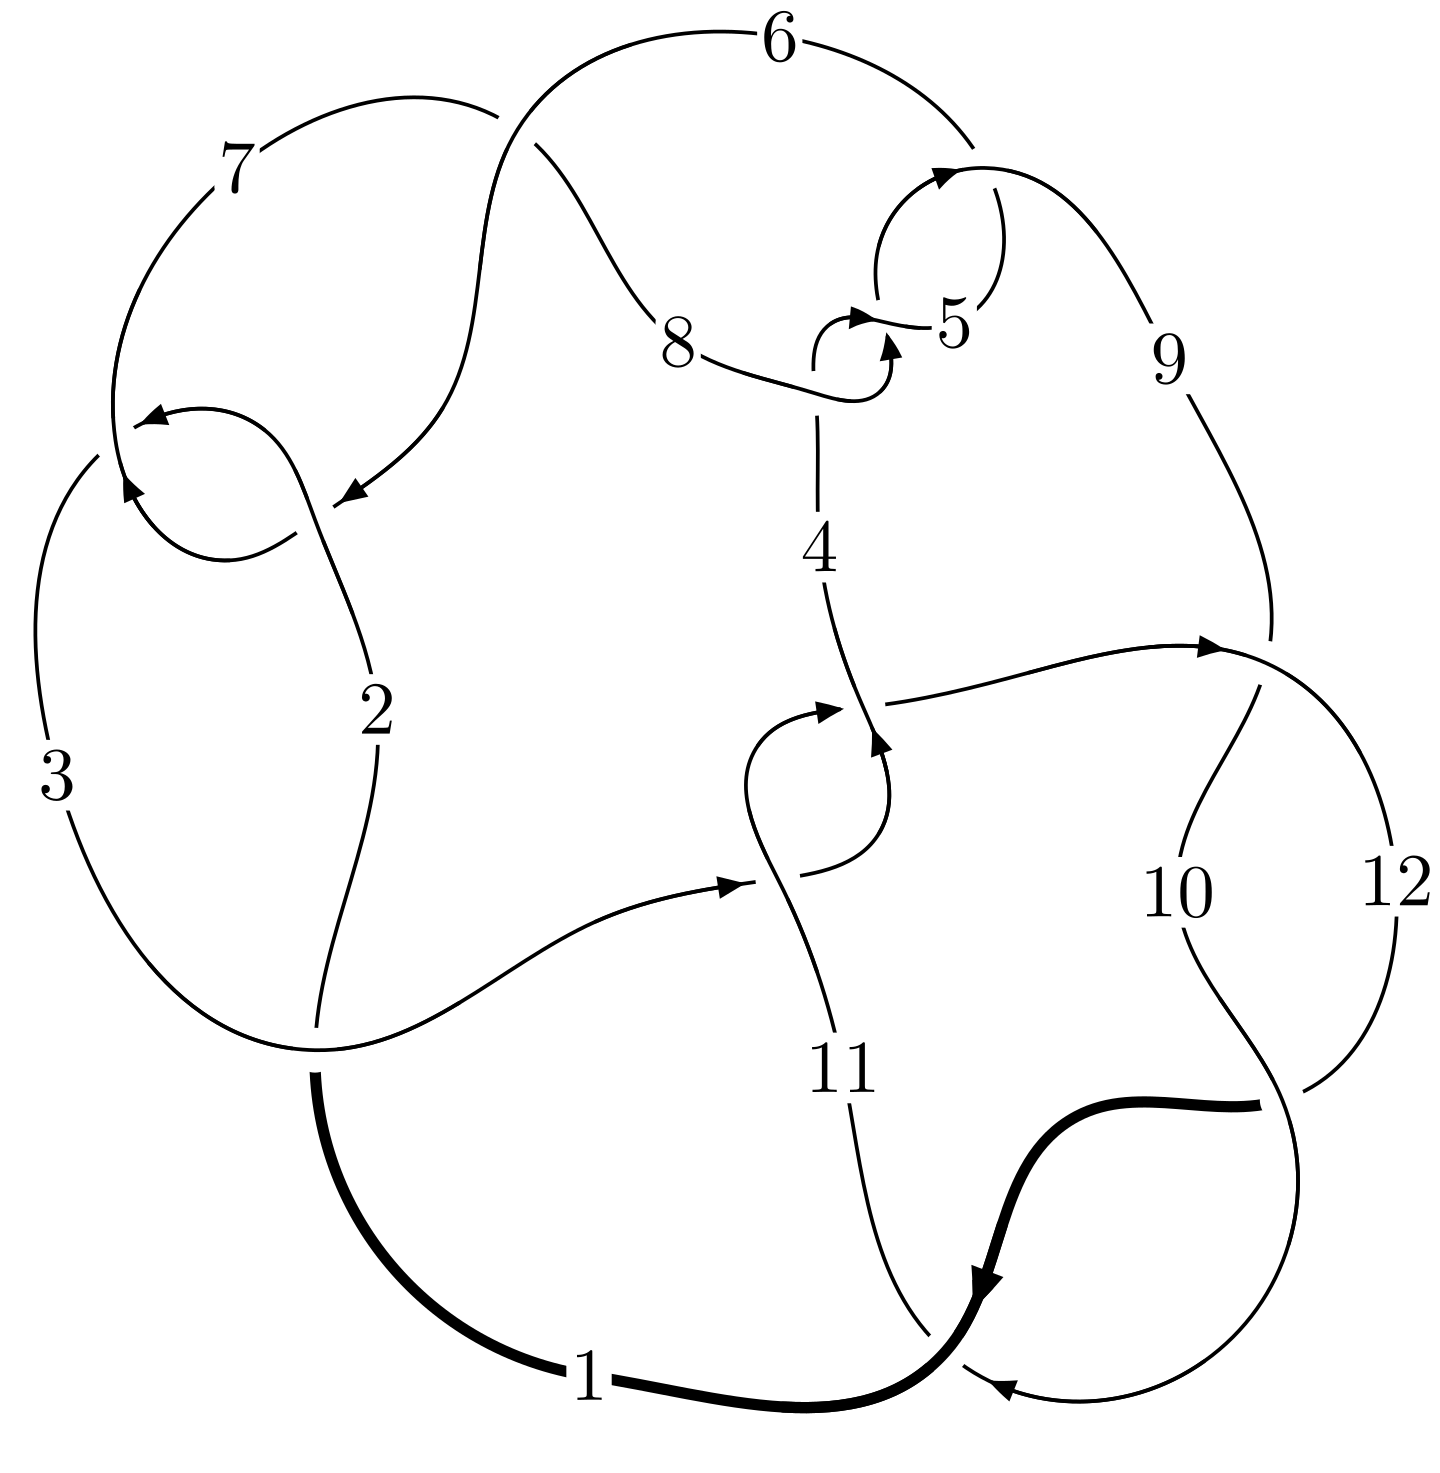
\includegraphics[width=112pt]{../../../GIT/diagram.site/Diagrams/png/1468_12a_0667.png}\\
\ \ \ A knot diagram\footnotemark}&
\allowdisplaybreaks
\textbf{Linearized knot diagam} \\
\cline{2-2}
 &
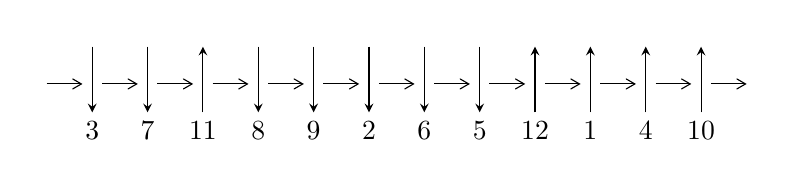
\begin{tikzpicture}[x=20pt, y=17pt]
	% nodes
	\node (C0) at (0, 0) {};
	\node (C1) at (1, 0) {};
	\node (C1U) at (1, +1) {};
	\node (C1D) at (1, -1) {3};

	\node (C2) at (2, 0) {};
	\node (C2U) at (2, +1) {};
	\node (C2D) at (2, -1) {7};

	\node (C3) at (3, 0) {};
	\node (C3U) at (3, +1) {};
	\node (C3D) at (3, -1) {11};

	\node (C4) at (4, 0) {};
	\node (C4U) at (4, +1) {};
	\node (C4D) at (4, -1) {8};

	\node (C5) at (5, 0) {};
	\node (C5U) at (5, +1) {};
	\node (C5D) at (5, -1) {9};

	\node (C6) at (6, 0) {};
	\node (C6U) at (6, +1) {};
	\node (C6D) at (6, -1) {2};

	\node (C7) at (7, 0) {};
	\node (C7U) at (7, +1) {};
	\node (C7D) at (7, -1) {6};

	\node (C8) at (8, 0) {};
	\node (C8U) at (8, +1) {};
	\node (C8D) at (8, -1) {5};

	\node (C9) at (9, 0) {};
	\node (C9U) at (9, +1) {};
	\node (C9D) at (9, -1) {12};

	\node (C10) at (10, 0) {};
	\node (C10U) at (10, +1) {};
	\node (C10D) at (10, -1) {1};

	\node (C11) at (11, 0) {};
	\node (C11U) at (11, +1) {};
	\node (C11D) at (11, -1) {4};

	\node (C12) at (12, 0) {};
	\node (C12U) at (12, +1) {};
	\node (C12D) at (12, -1) {10};
	\node (C13) at (13, 0) {};

	% arrows
	\draw[->,>={angle 60}]
	(C0) edge (C1) (C1) edge (C2) (C2) edge (C3) (C3) edge (C4) (C4) edge (C5) (C5) edge (C6) (C6) edge (C7) (C7) edge (C8) (C8) edge (C9) (C9) edge (C10) (C10) edge (C11) (C11) edge (C12) (C12) edge (C13) ;	\draw[->,>=stealth]
	(C1U) edge (C1D) (C2U) edge (C2D) (C3D) edge (C3U) (C4U) edge (C4D) (C5U) edge (C5D) (C6U) edge (C6D) (C7U) edge (C7D) (C8U) edge (C8D) (C9D) edge (C9U) (C10D) edge (C10U) (C11D) edge (C11U) (C12D) edge (C12U) ;
	\end{tikzpicture} \\
\hhline{~~} \\& 
\textbf{Solving Sequence} \\ \cline{2-2} 
 &
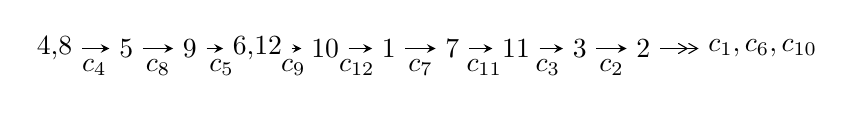
\begin{tikzpicture}[x=23pt, y=7pt]
	% node
	\node (A0) at (-1/8, 0) {4,8};
	\node (A1) at (1, 0) {5};
	\node (A2) at (2, 0) {9};
	\node (A3) at (49/16, 0) {6,12};
	\node (A4) at (33/8, 0) {10};
	\node (A5) at (41/8, 0) {1};
	\node (A6) at (49/8, 0) {7};
	\node (A7) at (57/8, 0) {11};
	\node (A8) at (65/8, 0) {3};
	\node (A9) at (73/8, 0) {2};
	\node (C1) at (1/2, -1) {$c_{4}$};
	\node (C2) at (3/2, -1) {$c_{8}$};
	\node (C3) at (5/2, -1) {$c_{5}$};
	\node (C4) at (29/8, -1) {$c_{9}$};
	\node (C5) at (37/8, -1) {$c_{12}$};
	\node (C6) at (45/8, -1) {$c_{7}$};
	\node (C7) at (53/8, -1) {$c_{11}$};
	\node (C8) at (61/8, -1) {$c_{3}$};
	\node (C9) at (69/8, -1) {$c_{2}$};
	\node (A10) at (11, 0) {$c_{1},c_{6},c_{10}$};

	% edge
	\draw[->,>=stealth]	
	(A0) edge (A1) (A1) edge (A2) (A2) edge (A3) (A3) edge (A4) (A4) edge (A5) (A5) edge (A6) (A6) edge (A7) (A7) edge (A8) (A8) edge (A9) ;
	\draw[->>,>={angle 60}]	
	(A9) edge (A10);
\end{tikzpicture} \\ 

\end{tabular} \\

\footnotetext{
The image of knot diagram is generated by the software ``\textbf{Draw programme}" developed by Andrew Bartholomew(\url{http://www.layer8.co.uk/maths/draw/index.htm\#Running-draw}), where we modified some parts for our purpose(\url{https://github.com/CATsTAILs/LinksPainter}).
}\phantom \\ \newline 
\centering \textbf{Ideals for irreducible components\footnotemark of $X_{\text{par}}$} 
 
\begin{align*}
I^u_{1}&=\langle 
-6.17038\times10^{20} u^{69}-1.82582\times10^{21} u^{68}+\cdots+1.91455\times10^{20} b-4.81975\times10^{20},\\
\phantom{I^u_{1}}&\phantom{= \langle  }-8.95967\times10^{20} u^{69}-2.35544\times10^{21} u^{68}+\cdots+9.57277\times10^{19} a-1.80647\times10^{21},\\
\phantom{I^u_{1}}&\phantom{= \langle  }u^{70}+4 u^{69}+\cdots-12 u+1\rangle \\
I^u_{2}&=\langle 
b,\;- u^7-2 u^6+2 u^5+4 u^4-2 u^3- u^2+a+u-3,\;u^8+u^7-3 u^6-2 u^5+3 u^4+2 u-1\rangle \\
I^u_{3}&=\langle 
b^2+b-1,\;a+1,\;u-1\rangle \\
\\
\end{align*}
\raggedright * 3 irreducible components of $\dim_{\mathbb{C}}=0$, with total 80 representations.\\
\footnotetext{All coefficients of polynomials are rational numbers. But the coefficients are sometimes approximated in decimal forms when there is not enough margin.}
\newpage
\renewcommand{\arraystretch}{1}
\centering \section*{I. $I^u_{1}= \langle -6.17\times10^{20} u^{69}-1.83\times10^{21} u^{68}+\cdots+1.91\times10^{20} b-4.82\times10^{20},\;-8.96\times10^{20} u^{69}-2.36\times10^{21} u^{68}+\cdots+9.57\times10^{19} a-1.81\times10^{21},\;u^{70}+4 u^{69}+\cdots-12 u+1 \rangle$}
\flushleft \textbf{(i) Arc colorings}\\
\begin{tabular}{m{7pt} m{180pt} m{7pt} m{180pt} }
\flushright $a_{4}=$&$\begin{pmatrix}1\\0\end{pmatrix}$ \\
\flushright $a_{8}=$&$\begin{pmatrix}0\\u\end{pmatrix}$ \\
\flushright $a_{5}=$&$\begin{pmatrix}1\\u^2\end{pmatrix}$ \\
\flushright $a_{9}=$&$\begin{pmatrix}- u\\- u^3+u\end{pmatrix}$ \\
\flushright $a_{6}=$&$\begin{pmatrix}- u^2+1\\- u^4+2 u^2\end{pmatrix}$ \\
\flushright $a_{12}=$&$\begin{pmatrix}9.35954 u^{69}+24.6057 u^{68}+\cdots-158.582 u+18.8709\\3.22288 u^{69}+9.53652 u^{68}+\cdots-38.9678 u+2.51743\end{pmatrix}$ \\
\flushright $a_{10}=$&$\begin{pmatrix}10.8850 u^{69}+29.1016 u^{68}+\cdots-165.811 u+18.2326\\0.777120 u^{69}+2.46348 u^{68}+\cdots-10.0322 u+0.482574\end{pmatrix}$ \\
\flushright $a_{1}=$&$\begin{pmatrix}-5.12581 u^{69}-14.9838 u^{68}+\cdots+40.9018 u-1.06043\\0.777120 u^{69}+2.46348 u^{68}+\cdots-10.0322 u+0.482574\end{pmatrix}$ \\
\flushright $a_{7}=$&$\begin{pmatrix}u^5-2 u^3+u\\u^7-3 u^5+2 u^3+u\end{pmatrix}$ \\
\flushright $a_{11}=$&$\begin{pmatrix}6.13666 u^{69}+15.0692 u^{68}+\cdots-119.615 u+16.3535\\3.22288 u^{69}+9.53652 u^{68}+\cdots-38.9678 u+2.51743\end{pmatrix}$ \\
\flushright $a_{3}=$&$\begin{pmatrix}-4.34064 u^{69}-10.9959 u^{68}+\cdots+62.9281 u-7.39444\\-1.66141 u^{69}-5.91374 u^{68}+\cdots+28.6144 u-1.97273\end{pmatrix}$ \\
\flushright $a_{2}=$&$\begin{pmatrix}0.857437 u^{69}+3.79945 u^{68}+\cdots+1.94293 u-2.59562\\3.53647 u^{69}+7.44091 u^{68}+\cdots-20.9351 u+1.99464\end{pmatrix}$\\&\end{tabular}
\flushleft \textbf{(ii) Obstruction class $= -1$}\\~\\
\flushleft \textbf{(iii) Cusp Shapes $= \frac{407739505172525880142}{95727673049700434881} u^{69}+\frac{445100059269514406149}{95727673049700434881} u^{68}+\cdots-\frac{14149863699302255302262}{95727673049700434881} u+\frac{2264603463256005582788}{95727673049700434881}$}\\~\\
\newpage\renewcommand{\arraystretch}{1}
\flushleft \textbf{(iv) u-Polynomials at the component}\newline \\
\begin{tabular}{m{50pt}|m{274pt}}
Crossings & \hspace{64pt}u-Polynomials at each crossing \\
\hline $$\begin{aligned}c_{1},c_{7}\end{aligned}$$&$\begin{aligned}
&u^{70}+18 u^{69}+\cdots+392 u+16
\end{aligned}$\\
\hline $$\begin{aligned}c_{2},c_{6}\end{aligned}$$&$\begin{aligned}
&u^{70}-2 u^{69}+\cdots-4 u+4
\end{aligned}$\\
\hline $$\begin{aligned}c_{3},c_{11}\end{aligned}$$&$\begin{aligned}
&u^{70}-2 u^{69}+\cdots-128 u+256
\end{aligned}$\\
\hline $$\begin{aligned}c_{4},c_{5},c_{8}\end{aligned}$$&$\begin{aligned}
&u^{70}-4 u^{69}+\cdots+12 u+1
\end{aligned}$\\
\hline $$\begin{aligned}c_{9},c_{10},c_{12}\end{aligned}$$&$\begin{aligned}
&u^{70}+10 u^{69}+\cdots- u+1
\end{aligned}$\\
\hline
\end{tabular}\\~\\
\newpage\renewcommand{\arraystretch}{1}
\flushleft \textbf{(v) Riley Polynomials at the component}\newline \\
\begin{tabular}{m{50pt}|m{274pt}}
Crossings & \hspace{64pt}Riley Polynomials at each crossing \\
\hline $$\begin{aligned}c_{1},c_{7}\end{aligned}$$&$\begin{aligned}
&y^{70}+66 y^{69}+\cdots-11552 y+256
\end{aligned}$\\
\hline $$\begin{aligned}c_{2},c_{6}\end{aligned}$$&$\begin{aligned}
&y^{70}-18 y^{69}+\cdots-392 y+16
\end{aligned}$\\
\hline $$\begin{aligned}c_{3},c_{11}\end{aligned}$$&$\begin{aligned}
&y^{70}-54 y^{69}+\cdots-573440 y+65536
\end{aligned}$\\
\hline $$\begin{aligned}c_{4},c_{5},c_{8}\end{aligned}$$&$\begin{aligned}
&y^{70}-56 y^{69}+\cdots-16 y+1
\end{aligned}$\\
\hline $$\begin{aligned}c_{9},c_{10},c_{12}\end{aligned}$$&$\begin{aligned}
&y^{70}-74 y^{69}+\cdots-29 y+1
\end{aligned}$\\
\hline
\end{tabular}\\~\\
\newpage\flushleft \textbf{(vi) Complex Volumes and Cusp Shapes}
$$\begin{array}{c|c|c}  
\text{Solutions to }I^u_{1}& \I (\text{vol} + \sqrt{-1}CS) & \text{Cusp shape}\\
 \hline 
\begin{aligned}
u &= \phantom{-}0.817401 + 0.528957 I \\
a &= -0.697679 + 0.470803 I \\
b &= -1.269240 - 0.137383 I\end{aligned}
 & \phantom{-}4.41806 + 0.85765 I & \phantom{-0.000000 } 0 \\ \hline\begin{aligned}
u &= \phantom{-}0.817401 - 0.528957 I \\
a &= -0.697679 - 0.470803 I \\
b &= -1.269240 + 0.137383 I\end{aligned}
 & \phantom{-}4.41806 - 0.85765 I & \phantom{-0.000000 } 0 \\ \hline\begin{aligned}
u &= \phantom{-}0.092064 + 0.919453 I \\
a &= \phantom{-}0.846984 + 0.675426 I \\
b &= -1.51562 + 0.63048 I\end{aligned}
 & \phantom{-}13.9368 - 10.3001 I & \phantom{-}4.79104 + 5.95830 I \\ \hline\begin{aligned}
u &= \phantom{-}0.092064 - 0.919453 I \\
a &= \phantom{-}0.846984 - 0.675426 I \\
b &= -1.51562 - 0.63048 I\end{aligned}
 & \phantom{-}13.9368 + 10.3001 I & \phantom{-}4.79104 - 5.95830 I \\ \hline\begin{aligned}
u &= \phantom{-}1.104440 + 0.096151 I \\
a &= -0.13603 + 3.19897 I \\
b &= \phantom{-}0.257699 + 0.472682 I\end{aligned}
 & -0.029984 - 0.580196 I & \phantom{-0.000000 } 0 \\ \hline\begin{aligned}
u &= \phantom{-}1.104440 - 0.096151 I \\
a &= -0.13603 - 3.19897 I \\
b &= \phantom{-}0.257699 - 0.472682 I\end{aligned}
 & -0.029984 + 0.580196 I & \phantom{-0.000000 } 0 \\ \hline\begin{aligned}
u &= -1.11750\phantom{ +0.000000I} \\
a &= \phantom{-}0.916637\phantom{ +0.000000I} \\
b &= \phantom{-}1.71816\phantom{ +0.000000I}\end{aligned}
 & \phantom{-}6.85417\phantom{ +0.000000I} & \phantom{-0.000000 } 0 \\ \hline\begin{aligned}
u &= \phantom{-}0.062255 + 0.875793 I \\
a &= -1.267380 - 0.330024 I \\
b &= \phantom{-}1.322790 - 0.267712 I\end{aligned}
 & \phantom{-}6.93192 - 5.96613 I & \phantom{-}3.25852 + 5.54743 I \\ \hline\begin{aligned}
u &= \phantom{-}0.062255 - 0.875793 I \\
a &= -1.267380 + 0.330024 I \\
b &= \phantom{-}1.322790 + 0.267712 I\end{aligned}
 & \phantom{-}6.93192 + 5.96613 I & \phantom{-}3.25852 - 5.54743 I \\ \hline\begin{aligned}
u &= \phantom{-}0.033826 + 0.870423 I \\
a &= \phantom{-}0.060066 - 0.195647 I \\
b &= -0.059201 - 1.381390 I\end{aligned}
 & \phantom{-}9.25108 - 3.13331 I & \phantom{-}4.39715 + 2.61893 I\\
 \hline 
 \end{array}$$\newpage$$\begin{array}{c|c|c}  
\text{Solutions to }I^u_{1}& \I (\text{vol} + \sqrt{-1}CS) & \text{Cusp shape}\\
 \hline 
\begin{aligned}
u &= \phantom{-}0.033826 - 0.870423 I \\
a &= \phantom{-}0.060066 + 0.195647 I \\
b &= -0.059201 + 1.381390 I\end{aligned}
 & \phantom{-}9.25108 + 3.13331 I & \phantom{-}4.39715 - 2.61893 I \\ \hline\begin{aligned}
u &= -0.057165 + 0.862768 I \\
a &= -0.958752 + 0.804540 I \\
b &= \phantom{-}1.56506 + 0.55688 I\end{aligned}
 & \phantom{-}14.5560 + 3.8421 I & \phantom{-}5.88746 - 1.13079 I \\ \hline\begin{aligned}
u &= -0.057165 - 0.862768 I \\
a &= -0.958752 - 0.804540 I \\
b &= \phantom{-}1.56506 - 0.55688 I\end{aligned}
 & \phantom{-}14.5560 - 3.8421 I & \phantom{-}5.88746 + 1.13079 I \\ \hline\begin{aligned}
u &= \phantom{-}0.010182 + 0.850415 I \\
a &= \phantom{-}1.350140 - 0.323162 I \\
b &= -1.323590 - 0.156129 I\end{aligned}
 & \phantom{-}7.15687 - 0.24094 I & \phantom{-}4.01638 - 0.21668 I \\ \hline\begin{aligned}
u &= \phantom{-}0.010182 - 0.850415 I \\
a &= \phantom{-}1.350140 + 0.323162 I \\
b &= -1.323590 + 0.156129 I\end{aligned}
 & \phantom{-}7.15687 + 0.24094 I & \phantom{-}4.01638 + 0.21668 I \\ \hline\begin{aligned}
u &= \phantom{-}0.375035 + 0.735499 I \\
a &= \phantom{-}0.059630 + 0.986262 I \\
b &= -1.272940 + 0.299722 I\end{aligned}
 & \phantom{-}5.73321 - 5.43269 I & \phantom{-}2.26764 + 6.32769 I \\ \hline\begin{aligned}
u &= \phantom{-}0.375035 - 0.735499 I \\
a &= \phantom{-}0.059630 - 0.986262 I \\
b &= -1.272940 - 0.299722 I\end{aligned}
 & \phantom{-}5.73321 + 5.43269 I & \phantom{-}2.26764 - 6.32769 I \\ \hline\begin{aligned}
u &= \phantom{-}0.819505\phantom{ +0.000000I} \\
a &= -0.555435\phantom{ +0.000000I} \\
b &= \phantom{-}0.476341\phantom{ +0.000000I}\end{aligned}
 & -1.06753\phantom{ +0.000000I} & -12.4450\phantom{ +0.000000I} \\ \hline\begin{aligned}
u &= \phantom{-}0.083907 + 0.778419 I \\
a &= \phantom{-}0.0072775 - 0.0342586 I \\
b &= \phantom{-}0.030796 + 0.592717 I\end{aligned}
 & \phantom{-}2.76619 - 2.72730 I & -3.14275 + 3.54347 I \\ \hline\begin{aligned}
u &= \phantom{-}0.083907 - 0.778419 I \\
a &= \phantom{-}0.0072775 + 0.0342586 I \\
b &= \phantom{-}0.030796 - 0.592717 I\end{aligned}
 & \phantom{-}2.76619 + 2.72730 I & -3.14275 - 3.54347 I\\
 \hline 
 \end{array}$$\newpage$$\begin{array}{c|c|c}  
\text{Solutions to }I^u_{1}& \I (\text{vol} + \sqrt{-1}CS) & \text{Cusp shape}\\
 \hline 
\begin{aligned}
u &= \phantom{-}1.222300 + 0.088016 I \\
a &= -0.89405 + 1.85771 I \\
b &= -0.677538 + 0.339165 I\end{aligned}
 & -2.29879 - 1.51453 I & \phantom{-0.000000 } 0 \\ \hline\begin{aligned}
u &= \phantom{-}1.222300 - 0.088016 I \\
a &= -0.89405 - 1.85771 I \\
b &= -0.677538 - 0.339165 I\end{aligned}
 & -2.29879 + 1.51453 I & \phantom{-0.000000 } 0 \\ \hline\begin{aligned}
u &= \phantom{-}1.192390 + 0.314674 I \\
a &= -0.633153 - 0.565521 I \\
b &= -0.031337 - 0.548172 I\end{aligned}
 & -0.598685 - 1.239580 I & \phantom{-0.000000 } 0 \\ \hline\begin{aligned}
u &= \phantom{-}1.192390 - 0.314674 I \\
a &= -0.633153 + 0.565521 I \\
b &= -0.031337 + 0.548172 I\end{aligned}
 & -0.598685 + 1.239580 I & \phantom{-0.000000 } 0 \\ \hline\begin{aligned}
u &= -1.273260 + 0.103339 I \\
a &= \phantom{-}0.193105 - 1.137600 I \\
b &= -0.976495 - 0.415875 I\end{aligned}
 & -2.87928 + 1.19855 I & \phantom{-0.000000 } 0 \\ \hline\begin{aligned}
u &= -1.273260 - 0.103339 I \\
a &= \phantom{-}0.193105 + 1.137600 I \\
b &= -0.976495 + 0.415875 I\end{aligned}
 & -2.87928 - 1.19855 I & \phantom{-0.000000 } 0 \\ \hline\begin{aligned}
u &= -1.221250 + 0.407858 I \\
a &= \phantom{-}0.766170 + 0.123778 I \\
b &= \phantom{-}1.62804 - 0.49593 I\end{aligned}
 & \phantom{-}10.96800 + 0.71316 I & \phantom{-0.000000 } 0 \\ \hline\begin{aligned}
u &= -1.221250 - 0.407858 I \\
a &= \phantom{-}0.766170 - 0.123778 I \\
b &= \phantom{-}1.62804 + 0.49593 I\end{aligned}
 & \phantom{-}10.96800 - 0.71316 I & \phantom{-0.000000 } 0 \\ \hline\begin{aligned}
u &= \phantom{-}1.216830 + 0.424213 I \\
a &= -0.065916 - 0.625238 I \\
b &= \phantom{-}1.273500 + 0.190068 I\end{aligned}
 & \phantom{-}3.37423 + 1.31428 I & \phantom{-0.000000 } 0 \\ \hline\begin{aligned}
u &= \phantom{-}1.216830 - 0.424213 I \\
a &= -0.065916 + 0.625238 I \\
b &= \phantom{-}1.273500 - 0.190068 I\end{aligned}
 & \phantom{-}3.37423 - 1.31428 I & \phantom{-0.000000 } 0\\
 \hline 
 \end{array}$$\newpage$$\begin{array}{c|c|c}  
\text{Solutions to }I^u_{1}& \I (\text{vol} + \sqrt{-1}CS) & \text{Cusp shape}\\
 \hline 
\begin{aligned}
u &= \phantom{-}1.202860 + 0.484691 I \\
a &= -0.732064 + 0.135694 I \\
b &= -1.51639 - 0.56369 I\end{aligned}
 & \phantom{-}10.52640 + 5.31077 I & \phantom{-0.000000 } 0 \\ \hline\begin{aligned}
u &= \phantom{-}1.202860 - 0.484691 I \\
a &= -0.732064 - 0.135694 I \\
b &= -1.51639 + 0.56369 I\end{aligned}
 & \phantom{-}10.52640 - 5.31077 I & \phantom{-0.000000 } 0 \\ \hline\begin{aligned}
u &= -1.290110 + 0.161362 I \\
a &= -0.44688 + 1.68716 I \\
b &= -0.542031 + 0.941291 I\end{aligned}
 & -2.14802 + 3.82567 I & \phantom{-0.000000 } 0 \\ \hline\begin{aligned}
u &= -1.290110 - 0.161362 I \\
a &= -0.44688 - 1.68716 I \\
b &= -0.542031 - 0.941291 I\end{aligned}
 & -2.14802 - 3.82567 I & \phantom{-0.000000 } 0 \\ \hline\begin{aligned}
u &= \phantom{-}1.245330 + 0.412665 I \\
a &= \phantom{-}1.12163 + 1.42898 I \\
b &= \phantom{-}0.027402 + 1.331840 I\end{aligned}
 & \phantom{-}5.50508 - 1.46175 I & \phantom{-0.000000 } 0 \\ \hline\begin{aligned}
u &= \phantom{-}1.245330 - 0.412665 I \\
a &= \phantom{-}1.12163 - 1.42898 I \\
b &= \phantom{-}0.027402 - 1.331840 I\end{aligned}
 & \phantom{-}5.50508 + 1.46175 I & \phantom{-0.000000 } 0 \\ \hline\begin{aligned}
u &= \phantom{-}1.264760 + 0.391396 I \\
a &= \phantom{-}0.24842 + 1.62749 I \\
b &= -1.278590 + 0.241779 I\end{aligned}
 & \phantom{-}3.26582 - 4.21478 I & \phantom{-0.000000 } 0 \\ \hline\begin{aligned}
u &= \phantom{-}1.264760 - 0.391396 I \\
a &= \phantom{-}0.24842 - 1.62749 I \\
b &= -1.278590 - 0.241779 I\end{aligned}
 & \phantom{-}3.26582 + 4.21478 I & \phantom{-0.000000 } 0 \\ \hline\begin{aligned}
u &= -1.281160 + 0.389589 I \\
a &= \phantom{-}0.038433 - 0.693152 I \\
b &= -1.357220 + 0.068668 I\end{aligned}
 & \phantom{-}3.14091 + 4.69097 I & \phantom{-0.000000 } 0 \\ \hline\begin{aligned}
u &= -1.281160 - 0.389589 I \\
a &= \phantom{-}0.038433 + 0.693152 I \\
b &= -1.357220 - 0.068668 I\end{aligned}
 & \phantom{-}3.14091 - 4.69097 I & \phantom{-0.000000 } 0\\
 \hline 
 \end{array}$$\newpage$$\begin{array}{c|c|c}  
\text{Solutions to }I^u_{1}& \I (\text{vol} + \sqrt{-1}CS) & \text{Cusp shape}\\
 \hline 
\begin{aligned}
u &= -1.350210 + 0.062844 I \\
a &= \phantom{-}0.622603 - 1.117160 I \\
b &= \phantom{-}0.419600 - 0.660924 I\end{aligned}
 & -6.65005 + 1.01942 I & \phantom{-0.000000 } 0 \\ \hline\begin{aligned}
u &= -1.350210 - 0.062844 I \\
a &= \phantom{-}0.622603 + 1.117160 I \\
b &= \phantom{-}0.419600 + 0.660924 I\end{aligned}
 & -6.65005 - 1.01942 I & \phantom{-0.000000 } 0 \\ \hline\begin{aligned}
u &= \phantom{-}1.346040 + 0.140036 I \\
a &= \phantom{-}2.16278 - 1.54711 I \\
b &= \phantom{-}1.245680 - 0.222159 I\end{aligned}
 & \phantom{-}3.15551 - 3.32548 I & \phantom{-0.000000 } 0 \\ \hline\begin{aligned}
u &= \phantom{-}1.346040 - 0.140036 I \\
a &= \phantom{-}2.16278 + 1.54711 I \\
b &= \phantom{-}1.245680 + 0.222159 I\end{aligned}
 & \phantom{-}3.15551 + 3.32548 I & \phantom{-0.000000 } 0 \\ \hline\begin{aligned}
u &= -1.344330 + 0.179173 I \\
a &= \phantom{-}0.30073 + 1.60507 I \\
b &= \phantom{-}0.919661 + 0.547737 I\end{aligned}
 & -5.16563 + 5.58267 I & \phantom{-0.000000 } 0 \\ \hline\begin{aligned}
u &= -1.344330 - 0.179173 I \\
a &= \phantom{-}0.30073 - 1.60507 I \\
b &= \phantom{-}0.919661 - 0.547737 I\end{aligned}
 & -5.16563 - 5.58267 I & \phantom{-0.000000 } 0 \\ \hline\begin{aligned}
u &= -1.300510 + 0.401241 I \\
a &= -1.00810 + 1.38334 I \\
b &= -0.14268 + 1.40895 I\end{aligned}
 & \phantom{-}5.09074 + 7.69181 I & \phantom{-0.000000 } 0 \\ \hline\begin{aligned}
u &= -1.300510 - 0.401241 I \\
a &= -1.00810 - 1.38334 I \\
b &= -0.14268 - 1.40895 I\end{aligned}
 & \phantom{-}5.09074 - 7.69181 I & \phantom{-0.000000 } 0 \\ \hline\begin{aligned}
u &= -1.320910 + 0.336659 I \\
a &= \phantom{-}0.483780 - 0.643166 I \\
b &= \phantom{-}0.043065 - 0.637222 I\end{aligned}
 & -1.63951 + 6.75482 I & \phantom{-0.000000 } 0 \\ \hline\begin{aligned}
u &= -1.320910 - 0.336659 I \\
a &= \phantom{-}0.483780 + 0.643166 I \\
b &= \phantom{-}0.043065 + 0.637222 I\end{aligned}
 & -1.63951 - 6.75482 I & \phantom{-0.000000 } 0\\
 \hline 
 \end{array}$$\newpage$$\begin{array}{c|c|c}  
\text{Solutions to }I^u_{1}& \I (\text{vol} + \sqrt{-1}CS) & \text{Cusp shape}\\
 \hline 
\begin{aligned}
u &= \phantom{-}0.308688 + 0.550304 I \\
a &= -0.918995 - 0.683177 I \\
b &= \phantom{-}0.821372 - 0.340072 I\end{aligned}
 & \phantom{-0.000000 } -3.06118 I & -2.00068 + 8.85874 I \\ \hline\begin{aligned}
u &= \phantom{-}0.308688 - 0.550304 I \\
a &= -0.918995 + 0.683177 I \\
b &= \phantom{-}0.821372 + 0.340072 I\end{aligned}
 & \phantom{-0.000000 -}3.06118 I & -2.00068 - 8.85874 I \\ \hline\begin{aligned}
u &= \phantom{-}1.315760 + 0.392744 I \\
a &= \phantom{-}0.21638 - 2.33271 I \\
b &= \phantom{-}1.50161 - 0.59687 I\end{aligned}
 & \phantom{-}10.26400 - 8.34810 I & \phantom{-0.000000 } 0 \\ \hline\begin{aligned}
u &= \phantom{-}1.315760 - 0.392744 I \\
a &= \phantom{-}0.21638 + 2.33271 I \\
b &= \phantom{-}1.50161 + 0.59687 I\end{aligned}
 & \phantom{-}10.26400 + 8.34810 I & \phantom{-0.000000 } 0 \\ \hline\begin{aligned}
u &= -1.320220 + 0.400178 I \\
a &= -0.17686 + 1.53471 I \\
b &= \phantom{-}1.344730 + 0.338262 I\end{aligned}
 & \phantom{-}2.60924 + 10.54110 I & \phantom{-0.000000 } 0 \\ \hline\begin{aligned}
u &= -1.320220 - 0.400178 I \\
a &= -0.17686 - 1.53471 I \\
b &= \phantom{-}1.344730 - 0.338262 I\end{aligned}
 & \phantom{-}2.60924 - 10.54110 I & \phantom{-0.000000 } 0 \\ \hline\begin{aligned}
u &= -1.347670 + 0.419839 I \\
a &= -0.11657 - 2.13013 I \\
b &= -1.49498 - 0.68093 I\end{aligned}
 & \phantom{-}9.4229 + 15.0909 I & \phantom{-0.000000 } 0 \\ \hline\begin{aligned}
u &= -1.347670 - 0.419839 I \\
a &= -0.11657 + 2.13013 I \\
b &= -1.49498 + 0.68093 I\end{aligned}
 & \phantom{-}9.4229 - 15.0909 I & \phantom{-0.000000 } 0 \\ \hline\begin{aligned}
u &= \phantom{-}0.540431 + 0.219713 I \\
a &= -0.174418 - 0.008470 I \\
b &= \phantom{-}0.431863 + 0.284604 I\end{aligned}
 & -1.050260 - 0.096802 I & -9.26762 - 0.13740 I \\ \hline\begin{aligned}
u &= \phantom{-}0.540431 - 0.219713 I \\
a &= -0.174418 + 0.008470 I \\
b &= \phantom{-}0.431863 - 0.284604 I\end{aligned}
 & -1.050260 + 0.096802 I & -9.26762 + 0.13740 I\\
 \hline 
 \end{array}$$\newpage$$\begin{array}{c|c|c}  
\text{Solutions to }I^u_{1}& \I (\text{vol} + \sqrt{-1}CS) & \text{Cusp shape}\\
 \hline 
\begin{aligned}
u &= -1.41264 + 0.23660 I \\
a &= -1.12820 - 1.57936 I \\
b &= -1.171970 - 0.426637 I\end{aligned}
 & -0.02016 + 8.81445 I & \phantom{-0.000000 } 0 \\ \hline\begin{aligned}
u &= -1.41264 - 0.23660 I \\
a &= -1.12820 + 1.57936 I \\
b &= -1.171970 + 0.426637 I\end{aligned}
 & -0.02016 - 8.81445 I & \phantom{-0.000000 } 0 \\ \hline\begin{aligned}
u &= -1.45402\phantom{ +0.000000I} \\
a &= -1.76666\phantom{ +0.000000I} \\
b &= -1.04331\phantom{ +0.000000I}\end{aligned}
 & -3.23881\phantom{ +0.000000I} & \phantom{-0.000000 } 0 \\ \hline\begin{aligned}
u &= -0.324618 + 0.427664 I \\
a &= \phantom{-}0.66119 + 1.88807 I \\
b &= \phantom{-}1.44762 + 0.13518 I\end{aligned}
 & \phantom{-}8.35020 + 1.34425 I & \phantom{-}7.83795 - 1.26764 I \\ \hline\begin{aligned}
u &= -0.324618 - 0.427664 I \\
a &= \phantom{-}0.66119 - 1.88807 I \\
b &= \phantom{-}1.44762 - 0.13518 I\end{aligned}
 & \phantom{-}8.35020 - 1.34425 I & \phantom{-}7.83795 + 1.26764 I \\ \hline\begin{aligned}
u &= \phantom{-}0.176682 + 0.474018 I \\
a &= \phantom{-}0.89919 - 1.18021 I \\
b &= -0.249486 - 0.754350 I\end{aligned}
 & \phantom{-}2.34320 - 1.58119 I & \phantom{-}1.22087 + 3.59711 I \\ \hline\begin{aligned}
u &= \phantom{-}0.176682 - 0.474018 I \\
a &= \phantom{-}0.89919 + 1.18021 I \\
b &= -0.249486 + 0.754350 I\end{aligned}
 & \phantom{-}2.34320 + 1.58119 I & \phantom{-}1.22087 - 3.59711 I \\ \hline\begin{aligned}
u &= \phantom{-}0.031462 + 0.272546 I \\
a &= \phantom{-}1.94920 - 2.01252 I \\
b &= -0.736009 + 0.023221 I\end{aligned}
 & \phantom{-}1.228040 + 0.145895 I & \phantom{-}6.62969 + 0.43006 I \\ \hline\begin{aligned}
u &= \phantom{-}0.031462 - 0.272546 I \\
a &= \phantom{-}1.94920 + 2.01252 I \\
b &= -0.736009 - 0.023221 I\end{aligned}
 & \phantom{-}1.228040 - 0.145895 I & \phantom{-}6.62969 - 0.43006 I \\ \hline\begin{aligned}
u &= \phantom{-}0.154844\phantom{ +0.000000I} \\
a &= \phantom{-}6.14014\phantom{ +0.000000I} \\
b &= -0.481532\phantom{ +0.000000I}\end{aligned}
 & \phantom{-}1.16432\phantom{ +0.000000I} & \phantom{-}11.8160\phantom{ +0.000000I}\\
 \hline 
 \end{array}$$\newpage\newpage\renewcommand{\arraystretch}{1}
\centering \section*{II. $I^u_{2}= \langle b,\;- u^7-2 u^6+2 u^5+4 u^4-2 u^3- u^2+a+u-3,\;u^8+u^7-3 u^6-2 u^5+3 u^4+2 u-1 \rangle$}
\flushleft \textbf{(i) Arc colorings}\\
\begin{tabular}{m{7pt} m{180pt} m{7pt} m{180pt} }
\flushright $a_{4}=$&$\begin{pmatrix}1\\0\end{pmatrix}$ \\
\flushright $a_{8}=$&$\begin{pmatrix}0\\u\end{pmatrix}$ \\
\flushright $a_{5}=$&$\begin{pmatrix}1\\u^2\end{pmatrix}$ \\
\flushright $a_{9}=$&$\begin{pmatrix}- u\\- u^3+u\end{pmatrix}$ \\
\flushright $a_{6}=$&$\begin{pmatrix}- u^2+1\\- u^4+2 u^2\end{pmatrix}$ \\
\flushright $a_{12}=$&$\begin{pmatrix}u^7+2 u^6-2 u^5-4 u^4+2 u^3+u^2- u+3\\0\end{pmatrix}$ \\
\flushright $a_{10}=$&$\begin{pmatrix}u^7+2 u^6-2 u^5-4 u^4+2 u^3+u^2-2 u+3\\- u^3+u\end{pmatrix}$ \\
\flushright $a_{1}=$&$\begin{pmatrix}u\\u^3- u\end{pmatrix}$ \\
\flushright $a_{7}=$&$\begin{pmatrix}u^5-2 u^3+u\\u^7-3 u^5+2 u^3+u\end{pmatrix}$ \\
\flushright $a_{11}=$&$\begin{pmatrix}u^7+2 u^6-2 u^5-4 u^4+2 u^3+u^2- u+3\\0\end{pmatrix}$ \\
\flushright $a_{3}=$&$\begin{pmatrix}1\\0\end{pmatrix}$ \\
\flushright $a_{2}=$&$\begin{pmatrix}- u^3+2 u\\u^3- u\end{pmatrix}$\\&\end{tabular}
\flushleft \textbf{(ii) Obstruction class $= 1$}\\~\\
\flushleft \textbf{(iii) Cusp Shapes $= -3 u^7-10 u^6+7 u^5+25 u^4-9 u^3-12 u^2+8 u-13$}\\~\\
\newpage\renewcommand{\arraystretch}{1}
\flushleft \textbf{(iv) u-Polynomials at the component}\newline \\
\begin{tabular}{m{50pt}|m{274pt}}
Crossings & \hspace{64pt}u-Polynomials at each crossing \\
\hline $$\begin{aligned}c_{1}\end{aligned}$$&$\begin{aligned}
&u^8-3 u^7+7 u^6-10 u^5+11 u^4-10 u^3+6 u^2-4 u+1
\end{aligned}$\\
\hline $$\begin{aligned}c_{2}\end{aligned}$$&$\begin{aligned}
&u^8- u^7- u^6+2 u^5+u^4-2 u^3+2 u-1
\end{aligned}$\\
\hline $$\begin{aligned}c_{3},c_{11}\end{aligned}$$&$\begin{aligned}
&u^8
\end{aligned}$\\
\hline $$\begin{aligned}c_{4},c_{5}\end{aligned}$$&$\begin{aligned}
&u^8+u^7-3 u^6-2 u^5+3 u^4+2 u-1
\end{aligned}$\\
\hline $$\begin{aligned}c_{6}\end{aligned}$$&$\begin{aligned}
&u^8+u^7- u^6-2 u^5+u^4+2 u^3-2 u-1
\end{aligned}$\\
\hline $$\begin{aligned}c_{7}\end{aligned}$$&$\begin{aligned}
&u^8+3 u^7+7 u^6+10 u^5+11 u^4+10 u^3+6 u^2+4 u+1
\end{aligned}$\\
\hline $$\begin{aligned}c_{8}\end{aligned}$$&$\begin{aligned}
&u^8- u^7-3 u^6+2 u^5+3 u^4-2 u-1
\end{aligned}$\\
\hline $$\begin{aligned}c_{9},c_{10}\end{aligned}$$&$\begin{aligned}
&(u+1)^8
\end{aligned}$\\
\hline $$\begin{aligned}c_{12}\end{aligned}$$&$\begin{aligned}
&(u-1)^8
\end{aligned}$\\
\hline
\end{tabular}\\~\\
\newpage\renewcommand{\arraystretch}{1}
\flushleft \textbf{(v) Riley Polynomials at the component}\newline \\
\begin{tabular}{m{50pt}|m{274pt}}
Crossings & \hspace{64pt}Riley Polynomials at each crossing \\
\hline $$\begin{aligned}c_{1},c_{7}\end{aligned}$$&$\begin{aligned}
&y^8+5 y^7+11 y^6+6 y^5-17 y^4-34 y^3-22 y^2-4 y+1
\end{aligned}$\\
\hline $$\begin{aligned}c_{2},c_{6}\end{aligned}$$&$\begin{aligned}
&y^8-3 y^7+7 y^6-10 y^5+11 y^4-10 y^3+6 y^2-4 y+1
\end{aligned}$\\
\hline $$\begin{aligned}c_{3},c_{11}\end{aligned}$$&$\begin{aligned}
&y^8
\end{aligned}$\\
\hline $$\begin{aligned}c_{4},c_{5},c_{8}\end{aligned}$$&$\begin{aligned}
&y^8-7 y^7+19 y^6-22 y^5+3 y^4+14 y^3-6 y^2-4 y+1
\end{aligned}$\\
\hline $$\begin{aligned}c_{9},c_{10},c_{12}\end{aligned}$$&$\begin{aligned}
&(y-1)^8
\end{aligned}$\\
\hline
\end{tabular}\\~\\
\newpage\flushleft \textbf{(vi) Complex Volumes and Cusp Shapes}
$$\begin{array}{c|c|c}  
\text{Solutions to }I^u_{2}& \I (\text{vol} + \sqrt{-1}CS) & \text{Cusp shape}\\
 \hline 
\begin{aligned}
u &= \phantom{-}1.180120 + 0.268597 I \\
a &= -0.281371 + 1.128550 I \\
b &= \phantom{-0.000000 } 0\end{aligned}
 & \phantom{-}0.604279 - 1.131230 I & \phantom{-}2.43193 + 0.79885 I \\ \hline\begin{aligned}
u &= \phantom{-}1.180120 - 0.268597 I \\
a &= -0.281371 - 1.128550 I \\
b &= \phantom{-0.000000 } 0\end{aligned}
 & \phantom{-}0.604279 + 1.131230 I & \phantom{-}2.43193 - 0.79885 I \\ \hline\begin{aligned}
u &= \phantom{-}0.108090 + 0.747508 I \\
a &= \phantom{-}0.208670 - 0.825203 I \\
b &= \phantom{-0.000000 } 0\end{aligned}
 & \phantom{-}3.80435 - 2.57849 I & \phantom{-}5.57469 + 3.25625 I \\ \hline\begin{aligned}
u &= \phantom{-}0.108090 - 0.747508 I \\
a &= \phantom{-}0.208670 + 0.825203 I \\
b &= \phantom{-0.000000 } 0\end{aligned}
 & \phantom{-}3.80435 + 2.57849 I & \phantom{-}5.57469 - 3.25625 I \\ \hline\begin{aligned}
u &= -1.37100\phantom{ +0.000000I} \\
a &= \phantom{-}0.829189\phantom{ +0.000000I} \\
b &= \phantom{-0.000000 } 0\end{aligned}
 & -4.85780\phantom{ +0.000000I} & -8.00600\phantom{ +0.000000I} \\ \hline\begin{aligned}
u &= -1.334530 + 0.318930 I \\
a &= \phantom{-}0.284386 + 0.605794 I \\
b &= \phantom{-0.000000 } 0\end{aligned}
 & -0.73474 + 6.44354 I & \phantom{-}0.28408 - 3.92092 I \\ \hline\begin{aligned}
u &= -1.334530 - 0.318930 I \\
a &= \phantom{-}0.284386 - 0.605794 I \\
b &= \phantom{-0.000000 } 0\end{aligned}
 & -0.73474 - 6.44354 I & \phantom{-}0.28408 + 3.92092 I \\ \hline\begin{aligned}
u &= \phantom{-}0.463640\phantom{ +0.000000I} \\
a &= \phantom{-}2.74744\phantom{ +0.000000I} \\
b &= \phantom{-0.000000 } 0\end{aligned}
 & \phantom{-}0.799899\phantom{ +0.000000I} & -11.5750\phantom{ +0.000000I}\\
 \hline 
 \end{array}$$\newpage\newpage\renewcommand{\arraystretch}{1}
\centering \section*{III. $I^u_{3}= \langle b^2+b-1,\;a+1,\;u-1 \rangle$}
\flushleft \textbf{(i) Arc colorings}\\
\begin{tabular}{m{7pt} m{180pt} m{7pt} m{180pt} }
\flushright $a_{4}=$&$\begin{pmatrix}1\\0\end{pmatrix}$ \\
\flushright $a_{8}=$&$\begin{pmatrix}0\\1\end{pmatrix}$ \\
\flushright $a_{5}=$&$\begin{pmatrix}1\\1\end{pmatrix}$ \\
\flushright $a_{9}=$&$\begin{pmatrix}-1\\0\end{pmatrix}$ \\
\flushright $a_{6}=$&$\begin{pmatrix}0\\1\end{pmatrix}$ \\
\flushright $a_{12}=$&$\begin{pmatrix}-1\\b\end{pmatrix}$ \\
\flushright $a_{10}=$&$\begin{pmatrix}- b-1\\- b+1\end{pmatrix}$ \\
\flushright $a_{1}=$&$\begin{pmatrix}0\\- b+1\end{pmatrix}$ \\
\flushright $a_{7}=$&$\begin{pmatrix}0\\1\end{pmatrix}$ \\
\flushright $a_{11}=$&$\begin{pmatrix}- b-1\\b\end{pmatrix}$ \\
\flushright $a_{3}=$&$\begin{pmatrix}0\\- b+1\end{pmatrix}$ \\
\flushright $a_{2}=$&$\begin{pmatrix}0\\- b+1\end{pmatrix}$\\&\end{tabular}
\flushleft \textbf{(ii) Obstruction class $= 1$}\\~\\
\flushleft \textbf{(iii) Cusp Shapes $= 9$}\\~\\
\newpage\renewcommand{\arraystretch}{1}
\flushleft \textbf{(iv) u-Polynomials at the component}\newline \\
\begin{tabular}{m{50pt}|m{274pt}}
Crossings & \hspace{64pt}u-Polynomials at each crossing \\
\hline $$\begin{aligned}c_{1},c_{2},c_{6}\\c_{7}\end{aligned}$$&$\begin{aligned}
&u^2
\end{aligned}$\\
\hline $$\begin{aligned}c_{3},c_{12}\end{aligned}$$&$\begin{aligned}
&u^2+u-1
\end{aligned}$\\
\hline $$\begin{aligned}c_{4},c_{5}\end{aligned}$$&$\begin{aligned}
&(u-1)^2
\end{aligned}$\\
\hline $$\begin{aligned}c_{8}\end{aligned}$$&$\begin{aligned}
&(u+1)^2
\end{aligned}$\\
\hline $$\begin{aligned}c_{9},c_{10},c_{11}\end{aligned}$$&$\begin{aligned}
&u^2- u-1
\end{aligned}$\\
\hline
\end{tabular}\\~\\
\newpage\renewcommand{\arraystretch}{1}
\flushleft \textbf{(v) Riley Polynomials at the component}\newline \\
\begin{tabular}{m{50pt}|m{274pt}}
Crossings & \hspace{64pt}Riley Polynomials at each crossing \\
\hline $$\begin{aligned}c_{1},c_{2},c_{6}\\c_{7}\end{aligned}$$&$\begin{aligned}
&y^2
\end{aligned}$\\
\hline $$\begin{aligned}c_{3},c_{9},c_{10}\\c_{11},c_{12}\end{aligned}$$&$\begin{aligned}
&y^2-3 y+1
\end{aligned}$\\
\hline $$\begin{aligned}c_{4},c_{5},c_{8}\end{aligned}$$&$\begin{aligned}
&(y-1)^2
\end{aligned}$\\
\hline
\end{tabular}\\~\\
\newpage\flushleft \textbf{(vi) Complex Volumes and Cusp Shapes}
$$\begin{array}{c|c|c}  
\text{Solutions to }I^u_{3}& \I (\text{vol} + \sqrt{-1}CS) & \text{Cusp shape}\\
 \hline 
\begin{aligned}
u &= \phantom{-}1.00000\phantom{ +0.000000I} \\
a &= -1.00000\phantom{ +0.000000I} \\
b &= \phantom{-}0.618034\phantom{ +0.000000I}\end{aligned}
 & -0.657974\phantom{ +0.000000I} & \phantom{-}9.00000\phantom{ +0.000000I} \\ \hline\begin{aligned}
u &= \phantom{-}1.00000\phantom{ +0.000000I} \\
a &= -1.00000\phantom{ +0.000000I} \\
b &= -1.61803\phantom{ +0.000000I}\end{aligned}
 & \phantom{-}7.23771\phantom{ +0.000000I} & \phantom{-}9.00000\phantom{ +0.000000I}\\
 \hline 
 \end{array}$$\newpage
\newpage\renewcommand{\arraystretch}{1}
\centering \section*{ IV. u-Polynomials}
\begin{tabular}{m{50pt}|m{274pt}}
Crossings & \hspace{64pt}u-Polynomials at each crossing \\
\hline $$\begin{aligned}c_{1}\end{aligned}$$&$\begin{aligned}
&u^2(u^8-3 u^7+7 u^6-10 u^5+11 u^4-10 u^3+6 u^2-4 u+1)\\
&\cdot(u^{70}+18 u^{69}+\cdots+392 u+16)
\end{aligned}$\\
\hline $$\begin{aligned}c_{2}\end{aligned}$$&$\begin{aligned}
&u^2(u^8- u^7+\cdots+2 u-1)(u^{70}-2 u^{69}+\cdots-4 u+4)
\end{aligned}$\\
\hline $$\begin{aligned}c_{3}\end{aligned}$$&$\begin{aligned}
&u^8(u^2+u-1)(u^{70}-2 u^{69}+\cdots-128 u+256)
\end{aligned}$\\
\hline $$\begin{aligned}c_{4},c_{5}\end{aligned}$$&$\begin{aligned}
&(u-1)^2(u^8+u^7-3 u^6-2 u^5+3 u^4+2 u-1)\\
&\cdot(u^{70}-4 u^{69}+\cdots+12 u+1)
\end{aligned}$\\
\hline $$\begin{aligned}c_{6}\end{aligned}$$&$\begin{aligned}
&u^2(u^8+u^7+\cdots-2 u-1)(u^{70}-2 u^{69}+\cdots-4 u+4)
\end{aligned}$\\
\hline $$\begin{aligned}c_{7}\end{aligned}$$&$\begin{aligned}
&u^2(u^8+3 u^7+7 u^6+10 u^5+11 u^4+10 u^3+6 u^2+4 u+1)\\
&\cdot(u^{70}+18 u^{69}+\cdots+392 u+16)
\end{aligned}$\\
\hline $$\begin{aligned}c_{8}\end{aligned}$$&$\begin{aligned}
&(u+1)^2(u^8- u^7-3 u^6+2 u^5+3 u^4-2 u-1)\\
&\cdot(u^{70}-4 u^{69}+\cdots+12 u+1)
\end{aligned}$\\
\hline $$\begin{aligned}c_{9},c_{10}\end{aligned}$$&$\begin{aligned}
&((u+1)^8)(u^2- u-1)(u^{70}+10 u^{69}+\cdots- u+1)
\end{aligned}$\\
\hline $$\begin{aligned}c_{11}\end{aligned}$$&$\begin{aligned}
&u^8(u^2- u-1)(u^{70}-2 u^{69}+\cdots-128 u+256)
\end{aligned}$\\
\hline $$\begin{aligned}c_{12}\end{aligned}$$&$\begin{aligned}
&((u-1)^8)(u^2+u-1)(u^{70}+10 u^{69}+\cdots- u+1)
\end{aligned}$\\
\hline
\end{tabular}\newpage\renewcommand{\arraystretch}{1}
\centering \section*{ V. Riley Polynomials}
\begin{tabular}{m{50pt}|m{274pt}}
Crossings & \hspace{64pt}Riley Polynomials at each crossing \\
\hline $$\begin{aligned}c_{1},c_{7}\end{aligned}$$&$\begin{aligned}
&y^2(y^8+5 y^7+11 y^6+6 y^5-17 y^4-34 y^3-22 y^2-4 y+1)\\
&\cdot(y^{70}+66 y^{69}+\cdots-11552 y+256)
\end{aligned}$\\
\hline $$\begin{aligned}c_{2},c_{6}\end{aligned}$$&$\begin{aligned}
&y^2(y^8-3 y^7+7 y^6-10 y^5+11 y^4-10 y^3+6 y^2-4 y+1)\\
&\cdot(y^{70}-18 y^{69}+\cdots-392 y+16)
\end{aligned}$\\
\hline $$\begin{aligned}c_{3},c_{11}\end{aligned}$$&$\begin{aligned}
&y^8(y^2-3 y+1)(y^{70}-54 y^{69}+\cdots-573440 y+65536)
\end{aligned}$\\
\hline $$\begin{aligned}c_{4},c_{5},c_{8}\end{aligned}$$&$\begin{aligned}
&(y-1)^2(y^8-7 y^7+19 y^6-22 y^5+3 y^4+14 y^3-6 y^2-4 y+1)\\
&\cdot(y^{70}-56 y^{69}+\cdots-16 y+1)
\end{aligned}$\\
\hline $$\begin{aligned}c_{9},c_{10},c_{12}\end{aligned}$$&$\begin{aligned}
&((y-1)^8)(y^2-3 y+1)(y^{70}-74 y^{69}+\cdots-29 y+1)
\end{aligned}$\\
\hline
\end{tabular}
\vskip 2pc
\end{document}